\documentclass[12pt,a4paper]{article}

%------------------------------------------------
% Packages
%------------------------------------------------
\usepackage[T1]{fontenc}
\usepackage{lmodern}
\usepackage{graphicx}
\usepackage{amsmath,amssymb}
\usepackage{siunitx}
\usepackage{geometry}
\usepackage{fancyhdr}
\usepackage{booktabs}
\usepackage{caption}
\usepackage{float}
\usepackage{subcaption}
\usepackage{array}
\usepackage{setspace}
\usepackage[hidelinks]{hyperref}
\usepackage[backend=biber,style=numeric]{biblatex}

\addbibresource{references.bib}

%------------------------------------------------
% Page layout
%------------------------------------------------
\geometry{
    top=1in,
    bottom=1.2in,
    left=1in,
    right=1in
}

\setlength{\headheight}{15pt}
\setlength{\parskip}{0.4em}
\setlength{\parindent}{0pt}

\pagestyle{fancy}
\fancyhf{}
\fancyhead[L]{Ian Cullinane}
\fancyhead[R]{Millikan's Oil Drop Experiment}
\fancyfoot[C]{\thepage}

\sisetup{
    inter-unit-product = \cdot,
    uncertainty-mode = separate,
    per-mode = symbol
}

%------------------------------------------------
% Title
%------------------------------------------------
\title{
    \Large\textbf{Measuring the Elementary Charge with Millikan's Oil-Drop Method and Avogadro's Number}\\[0.5em]
    \large PY2107 -- Experiment 6
}

\author{
    Ian Cullinane -- \textit{125413342}\\[0.5em]
    Lab Partner: Fionn Lichtsinn Doyle\\[0.5em]
    Demonstrators: Jonathan and Olivia
}

\date{30th September 2026}

\begin{document}

\maketitle
\thispagestyle{empty}

\newpage
\tableofcontents
\newpage

%================================================
\section{Abstract}
%================================================

Millikan's 1913 oil-drop experiment was reproduced to test whether electric
charge is quantised and to measure the elementary charge $e$. The terminal
falling and rising speeds of 28 charged oil drops in air, with and without an
applied electric field, were used to determine each drop's radius and charge.
As in Millikan's original work, the charges did not form a continuum but fell
into three discrete levels, $n=1,2,3$, in the ratio $1:1.94:3.05$, close to
$1:2:3$. Millikan's central step, the slip (Cunningham) correction for drops
comparable in size to the mean free path of air, was applied with
$A=1.188$, calculated from the Leybold slip constant and a molecular diameter
of \SI{0.370}{nm}. This gives $e=(1.7\pm0.1)\times10^{-19}\,\si{C}$, in
agreement with the accepted value of $1.602\times10^{-19}\,\si{C}$ and with
Millikan's own result of approximately $1.59\times10^{-19}\,\si{C}$. Fitting
$A$ to the data, as Millikan did, gives $A=0.69\pm0.55$, consistent with the
analytic value within $0.9\sigma$ but too weakly constrained to test it. This
fitted $A$ implies $N_{\mathrm{A}}=(3.5\pm2.8)\times10^{23}\,\si{mol^{-1}}$,
consistent with the accepted value.

\newpage

%================================================
\section{Theory}
%================================================

An oil drop falling through air experiences gravity and viscous drag. As in
the lab briefing, buoyancy is neglected because the oil density is much
greater than the air density ($\rho_{oil} \gg \rho_{air}$). The gravitational force is therefore

\begin{equation}
    F_g = \frac{4}{3}\pi r^3\rho g,
\end{equation}

where $r$ is the drop radius and $\rho$ is the oil density. For a small
spherical drop, Stokes' law is corrected for non-continuum flow using the
Cunningham correction factor, following Cunningham's analysis of small
spherical particles moving through gases~\cite{cunningham1910}. A first order correction term is used as detailed in Appendix~\ref{app:cunningham}.

\begin{equation}
    C_{\mathrm{c}}(r,p) = 1 + \frac{b}{rp}
    = 1 + \frac{A}{r},
    \qquad A=\frac{b}{p},
\end{equation}

where $p$ is the air pressure, $b=80\,\mu\mathrm{m\,hPa}$ is the constant
specified for the Leybold apparatus, and $A$ is the pressure-dependent slip
length. Oxford independently reports $b=7.88\times10^{-3}\,\si{Pa.m}$,
consistent with the Leybold value $8.0\times10^{-3}\,\si{Pa.m}$ after unit
conversion~\cite{oxfordMillikan}. The corrected drag force is therefore

\begin{equation}
    F_D = \frac{6\pi\eta r v}{C_{\mathrm{c}}(r,p)}.
\end{equation}

Here $\eta$ is the viscosity of air and $v$ is the drop speed. The
pressure-dependent correction and its constant are given in the Leybold
apparatus documentation~\cite{leybold559412,oxfordMillikan}. With the electric field off,
a drop falling at terminal speed $v_g$ satisfies

\begin{equation}
    \frac{6\pi\eta r v_g}{C_{\mathrm{c}}(r,p)}
    = \frac{4}{3}\pi r^3\rho g,
    \label{eq:terminal-fall}
\end{equation}

giving us,

\begin{equation}
    r=\sqrt{\frac{9\eta v_g}{2\rho g}}.
    \label{eq:radius}
\end{equation}

When a potential difference $V$ is applied across plates separated by distance
$d$, the electric field is approximately $E=V/d$. The electric force on a
drop of charge $q$ is $F_E=qE$. If the drop rises at terminal speed $v_E$,
the electric force balances the drop's weight and the drag opposing the
upward motion. Combining the terminal-fall relation with the charge
force-balance gives the uncorrected charge $q_0$ and the Leybold slip-corrected
charge~\cite{leybold559412}:

\begin{equation}
    q_0 = \frac{4\pi d}{3V}
    \left(\frac{(9\eta/2)^3}{\rho g}\right)^{1/2}
    (v_g+v_E)\sqrt{v_g},
    \qquad
    q = \frac{q_0}{C_{\mathrm{c}}(r,p)^{3/2}}
    = \frac{q_0}{(1+A/r)^{3/2}}.
    \label{eq:drop-charge}
\end{equation}
For a stationary drop, $v_E=0$. Millikan's observation is that measured drop
charges occur in integer multiples of the elementary charge:
\begin{equation}
    q=ne,
\end{equation}
where $n$ is an integer and $e$ is the elementary charge, as observed by
Millikan~\cite{millikan1913}. A fit of $q$ against $n$ therefore estimates
$e$ from its slope.

When Millikan originally performed this experiment Cunningham's slip correction factor had been proposed 3 year earlier~\cite{cunningham1910}. Millikan was the first to measure its value.
His method involved plotting his apparent charge result before correction against the inverse radius as follow,
\begin{equation}
    q_{app}^{2/3} = q_1^{2/3}\left(q_1^{2/3} \cdot \frac{A\lambda}{r}\right)
    \label{eq:millikan-plot}
\end{equation}


\newpage

%================================================
\section{Experimental Procedure}
%================================================

A fine spray of oil was introduced into the region between the parallel
plates of the Leybold oil-drop apparatus. The plate separation was
$d=\SI{6}{mm}$, and each major graticule division represented
\SI{0.5}{mm}. Individual drops were observed through the microscope, and a
suitable drop was selected and followed as it moved through the field of
view. With the electric field switched off, the time taken to travel a known
distance was measured. This terminal falling speed, $v_g$, was used with
Equation~\ref{eq:terminal-fall} to determine the drop radius, including the
Cunningham correction for slip in the non-continuum regime.

A potential difference was then applied across the plates. The voltage and
the drop's motion were recorded, and its terminal rising speed $v_E$ (or zero
for a stationary drop) was determined over the measured distance. The falling
and rising speeds, plate separation, applied voltage, and calculated radius
were used in Equation~\ref{eq:drop-charge} to calculate the drop's charge.
This process was repeated for a number of drops. The resulting charges were
grouped by level, with each level corresponding to an integer multiple $n$ of
the elementary charge, and the charge-versus-level data were analysed to
estimate $e$.

\begin{figure}[H]
    \centering
    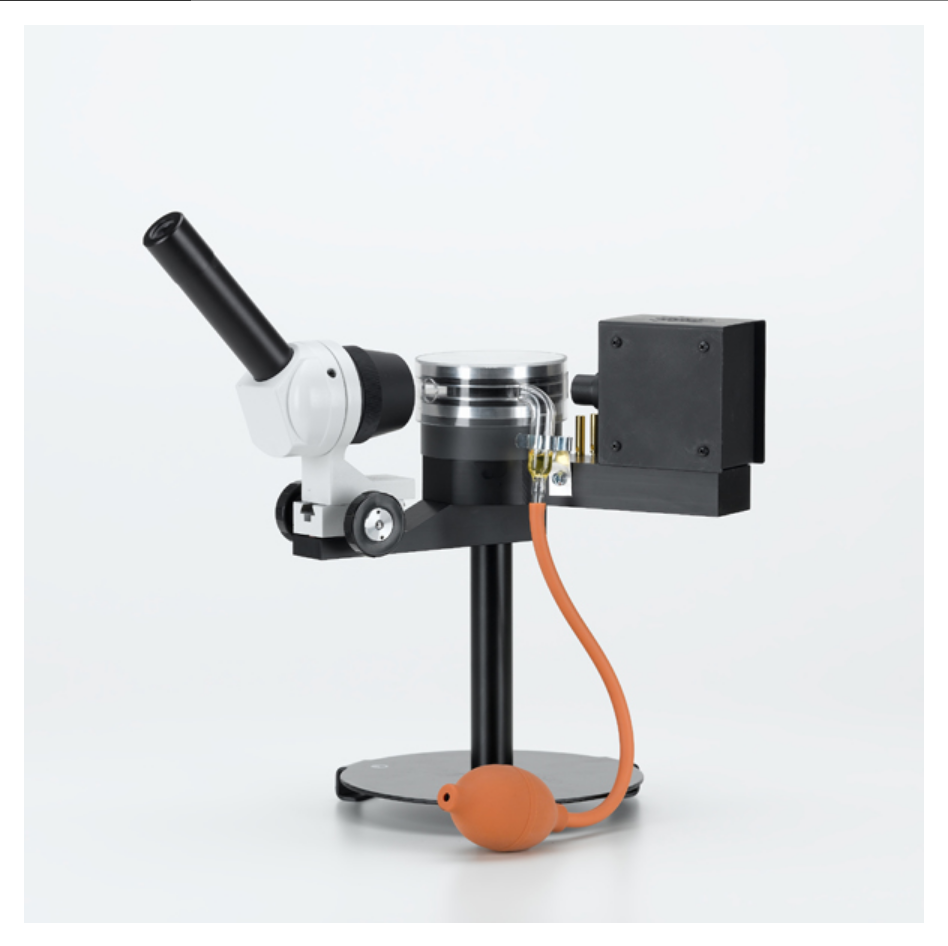
\includegraphics[width=0.8\textwidth]{images/Leybold_Apparatus.png}
    \caption{Leybold apparatus as used in this experiment}
    \label{fig:Apparatus}
\end{figure}

\begin{figure}[H]
    \centering
    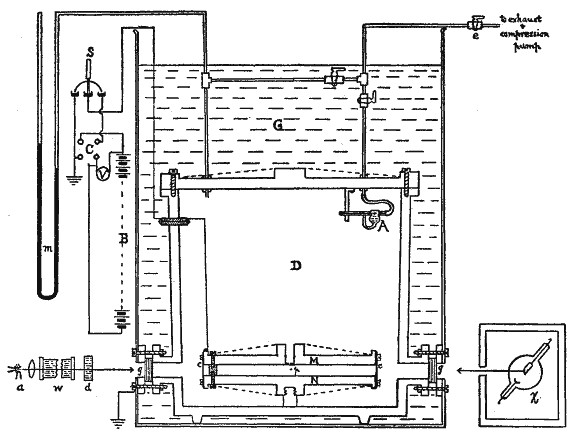
\includegraphics[width=0.8\textwidth]{images/Millikan_Apparatus.png}
    \caption{Diagram of the original apparatus as used by Millikan in 1913.}
    \label{fig:Millikan_Apparatus}
\end{figure}

\begin{figure}[H]
    \centering
    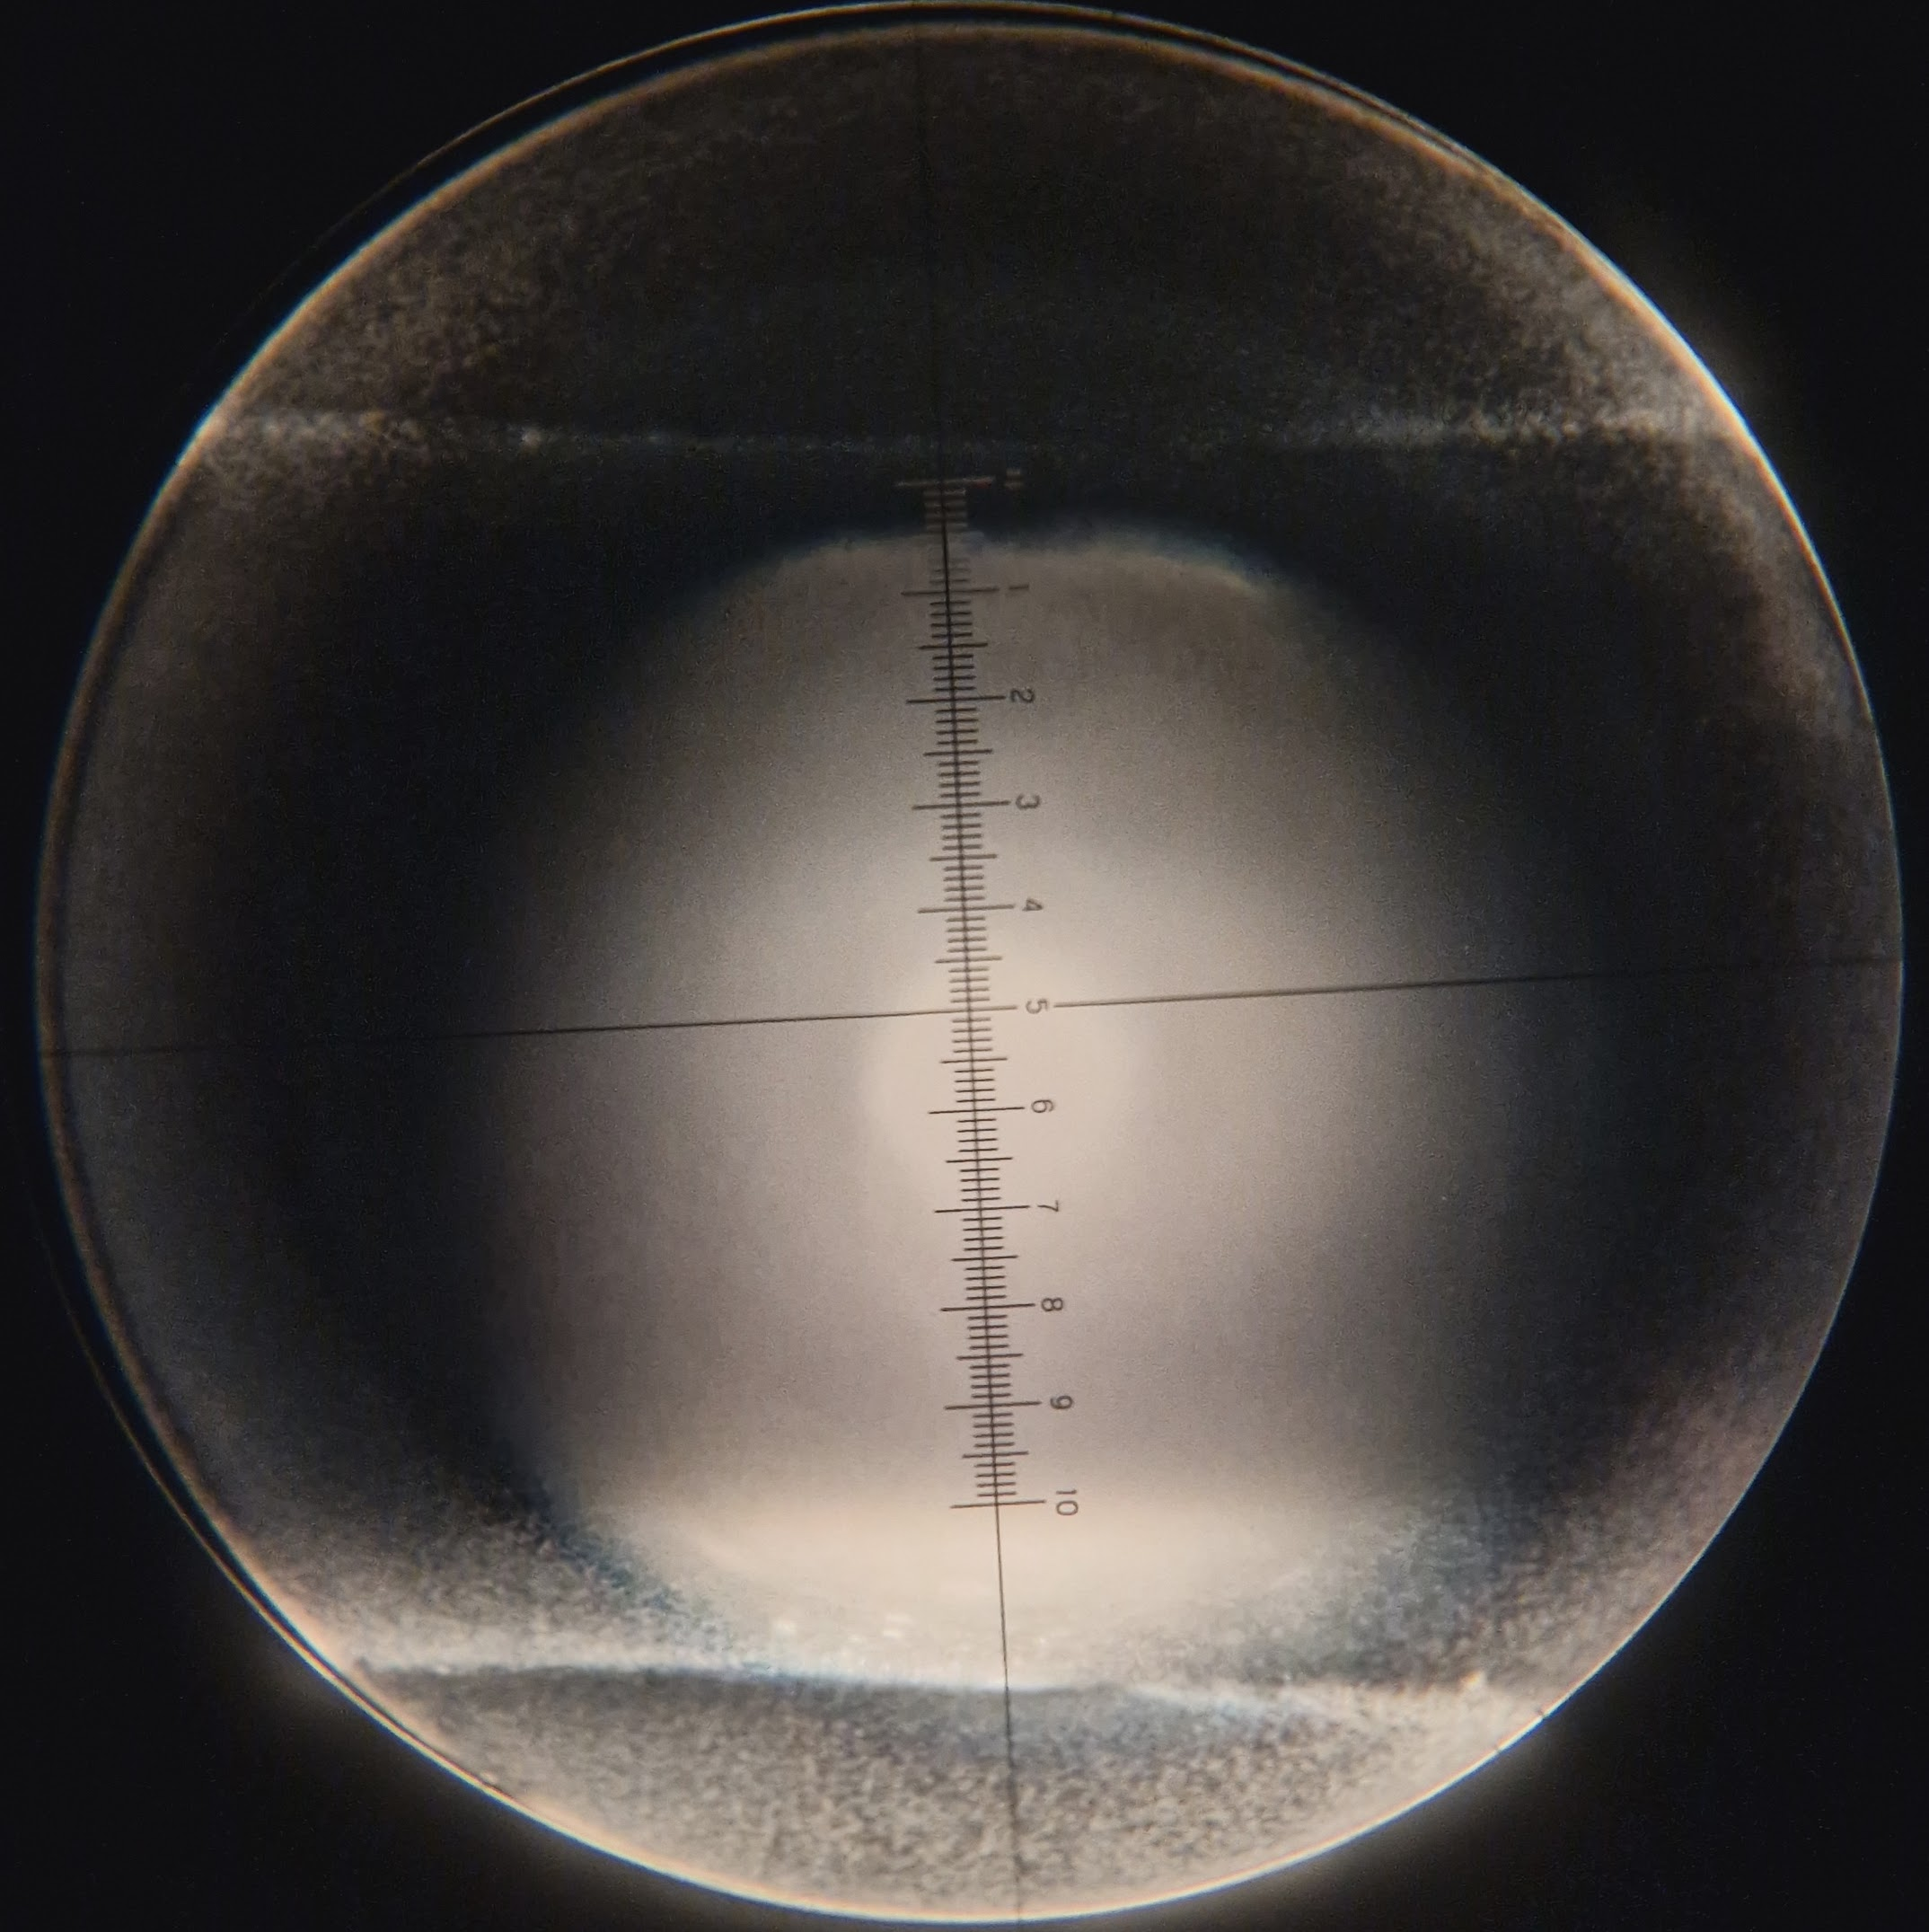
\includegraphics[width=0.8\textwidth]{images/Viewfinder.jpg}
    \caption{Viewfinder of the Leybold oil-drop apparatus. Contrast boosted. Drops visible on R.H.S.}
    \label{fig:Viewfinder}
\end{figure}

\newpage

%================================================
\section{Results}
%================================================

\begin{table}[H]
    \centering
    \caption{Summary of experimental parameters.}
    \begin{tabular}{|lll|}
    \hline
        Parameter & Symbol & Value \\ \hline
        Plate separation (treated as exact) & $d$ & \SI{6}{mm} \\
        Graticule division & $L$ & \SI{0.5}{mm} \\
        Temperature & $T$ & \SI{23.4 \pm 0.1}{C} \\
        Air viscosity (treated as exact) & $\eta$ & \SI{1.83e-5}{Pa.s} \\
        Oil density (treated as exact) & $\rho$ & \SI{900}{kg.m^{-3}} \\
        Slip constant (treated as exact) & $b$ & \SI{8.0e-3}{Pa.m} \\
        Atmospheric pressure & $P$ & \SI{1000 \pm 4}{hPa} \\ \hline
    \end{tabular}
    \centering
    \caption{Recomputed drop values with propagated one-standard-uncertainty errors. $v_E=0$ denotes a stationary drop. The first column gives the assigned charge level $n$.}
    \scriptsize
    \resizebox{\textwidth}{!}{%
    \begin{tabular}{ccccccc}
        \toprule
        Drop / $n$ & $v_g$ ($10^{-5}\,\si{m.s^{-1}}$) & $r$ ($10^{-7}\,\si{m}$) & $V$ ($\si{V}$) & $v_E$ ($10^{-5}\,\si{m.s^{-1}}$) & $q$ ($10^{-19}\,\si{C}$) & $q/n$ ($10^{-19}\,\si{C}$) \\
        \midrule
        1 / 1 & $5.282\pm0.880$ & $6.630\pm0.584$ & $573\pm0.5$ & $2.925\pm0.488$ & $1.754\pm0.374$ & $1.754\pm0.374$ \\
        2 / 1 & $5.474\pm0.912$ & $6.757\pm0.595$ & $568\pm0.5$ & $2.783\pm0.464$ & $1.818\pm0.391$ & $1.818\pm0.391$ \\
        3 / 3 & $11.565\pm1.928$ & $9.994\pm0.865$ & $418\pm0.5$ & $0$ & $5.299\pm1.376$ & $1.766\pm0.459$ \\
        4 / 1 & $4.820\pm0.803$ & $6.317\pm0.558$ & $327\pm0.5$ & $0$ & $1.711\pm0.453$ & $1.711\pm0.453$ \\
        5 / 1 & $4.820\pm0.803$ & $6.317\pm0.558$ & $565\pm0.5$ & $3.833\pm0.958$ & $1.777\pm0.392$ & $1.777\pm0.392$ \\
        6 / 1 & $5.144\pm0.857$ & $6.538\pm0.576$ & $345\pm0.5$ & $0$ & $1.798\pm0.475$ & $1.798\pm0.475$ \\
        7 / 1 & $5.144\pm0.857$ & $6.538\pm0.576$ & $572\pm0.5$ & $3.461\pm0.577$ & $1.814\pm0.378$ & $1.814\pm0.378$ \\
        8 / 2 & $5.334\pm0.889$ & $6.665\pm0.587$ & $193\pm0.5$ & $0$ & $3.404\pm0.899$ & $1.702\pm0.450$ \\
        9 / 3 & $8.170\pm1.362$ & $8.339\pm0.727$ & $233\pm0.5$ & $0$ & $5.522\pm1.444$ & $1.841\pm0.481$ \\
        10 / 3 & $8.170\pm1.362$ & $8.339\pm0.727$ & $578\pm0.5$ & $11.287\pm1.881$ & $5.301\pm1.013$ & $1.767\pm0.338$ \\
        11 / 3 & $8.170\pm1.362$ & $8.339\pm0.727$ & $350\pm0.5$ & $3.865\pm0.966$ & $5.415\pm1.207$ & $1.805\pm0.402$ \\
        12 / 1 & $5.369\pm0.895$ & $6.688\pm0.589$ & $578\pm0.5$ & $2.485\pm0.621$ & $1.680\pm0.379$ & $1.680\pm0.379$ \\
        13 / 1 & $6.053\pm1.009$ & $7.125\pm0.625$ & $460\pm0.5$ & $0$ & $1.745\pm0.459$ & $1.745\pm0.459$ \\
        14 / 1 & $6.053\pm1.009$ & $7.125\pm0.625$ & $578\pm0.5$ & $1.749\pm0.875$ & $1.790\pm0.451$ & $1.790\pm0.451$ \\
        15 / 1 & $5.503\pm0.917$ & $6.775\pm0.596$ & $578\pm0.5$ & $2.690\pm0.673$ & $1.778\pm0.400$ & $1.778\pm0.400$ \\
        16 / 1 & $5.710\pm0.952$ & $6.909\pm0.607$ & $407\pm0.5$ & $0$ & $1.798\pm0.474$ & $1.798\pm0.474$ \\
        17 / 3 & $10.115\pm1.686$ & $9.321\pm0.809$ & $333\pm0.5$ & $0$ & $5.397\pm1.405$ & $1.799\pm0.468$ \\
        18 / 3 & $10.115\pm1.686$ & $9.321\pm0.809$ & $578\pm0.5$ & $7.393\pm1.232$ & $5.382\pm1.090$ & $1.794\pm0.363$ \\
        19 / 2 & $8.586\pm1.431$ & $8.558\pm0.745$ & $578\pm0.5$ & $3.372\pm0.562$ & $3.351\pm0.735$ & $1.676\pm0.367$ \\
        20 / 2 & $8.586\pm1.431$ & $8.558\pm0.745$ & $382\pm0.5$ & $0$ & $3.641\pm0.951$ & $1.820\pm0.475$ \\
        21 / 1 & $5.803\pm0.967$ & $6.968\pm0.612$ & $438\pm0.5$ & $0$ & $1.714\pm0.452$ & $1.714\pm0.452$ \\
        22 / 1 & $5.803\pm0.967$ & $6.968\pm0.612$ & $578\pm0.5$ & $2.175\pm0.544$ & $1.785\pm0.408$ & $1.785\pm0.408$ \\
        23 / 1 & $4.088\pm0.681$ & $5.788\pm0.514$ & $246\pm0.5$ & $0$ & $1.749\pm0.466$ & $1.749\pm0.466$ \\
        24 / 1 & $4.088\pm0.681$ & $5.788\pm0.514$ & $591\pm0.5$ & $6.017\pm1.003$ & $1.800\pm0.349$ & $1.800\pm0.349$ \\
        25 / 2 & $5.503\pm0.917$ & $6.775\pm0.596$ & $590\pm0.5$ & $10.183\pm1.697$ & $3.334\pm0.632$ & $1.667\pm0.316$ \\
        26 / 2 & $5.503\pm0.917$ & $6.775\pm0.596$ & $208\pm0.5$ & $0$ & $3.318\pm0.876$ & $1.659\pm0.438$ \\
        27 / 2 & $5.938\pm0.990$ & $7.053\pm0.619$ & $590\pm0.5$ & $10.183\pm1.697$ & $3.582\pm0.681$ & $1.791\pm0.340$ \\
        28 / 2 & $5.938\pm0.990$ & $7.053\pm0.619$ & $227\pm0.5$ & $0$ & $3.430\pm0.903$ & $1.715\pm0.452$ \\ \hline
    \end{tabular}
    }
    \label{Results}
\end{table}

\newpage

%================================================
\section{Analysis}
%================================================

The charges were grouped into three observed levels and assigned integer
indices $n=1,2,3$, without using the accepted value of $e$ to set the levels.
The groups were identified by clustering the measured charges and ordered by
increasing mean charge. The mean charge at each level was divided by its index
to estimate $e$. The resulting estimates are summarised in
Table~\ref{tab:charge-levels}.

\begin{figure}[H]
    \centering
    \label{fig:measured-charge}
    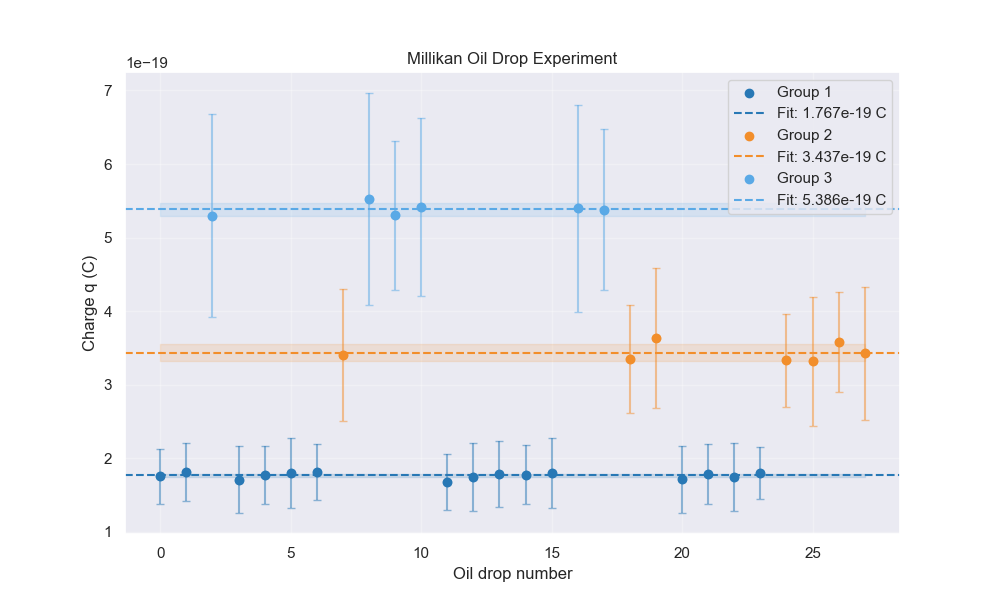
\includegraphics[width=0.8\textwidth]{images/Millikan_Oil_Drop_Experiment.png}
    \caption{Measured charge against drop number. Dashed horizontal lines show
    the mean charge of each group; this plot illustrates the three observed
    charge levels and is not the charge-versus-level fit used to estimate $e$.}
\end{figure}

\begin{table}[H]
    \centering
    \caption{Elementary-charge estimates obtained from each measurement level.}
    \begin{tabular}{lccc}
        \toprule
        Level & Measurements & $q$ (\si{C}) & $e=q/n$ (\si{C}) \\
        \midrule
        1 & 15 & $(1.7672 \pm 0.0106)\times10^{-19}$ & $(1.7672 \pm 0.0106)\times10^{-19}$ \\
        2 & 7  & $(3.4372 \pm 0.0478)\times10^{-19}$ & $(1.7186 \pm 0.0239)\times10^{-19}$ \\
        3 & 6  & $(5.3857 \pm 0.0338)\times10^{-19}$ & $(1.7952 \pm 0.0113)\times10^{-19}$ \\
        \bottomrule
    \end{tabular}
    \label{tab:charge-levels}
\end{table}

The weighted mean of the three level estimates is

\begin{equation}
    e_{\mathrm{weighted}} = (1.7745 \pm 0.0073)\times10^{-19}\,\si{C}.
\end{equation}

Using the propagated per-drop uncertainties and the shared pressure
uncertainty as a common covariance contribution, a generalised least-squares
fit of charge against the assigned integer $n$, as seen in fig.~\ref{fig:combined-analysis}, gives

\begin{equation}
    e = (1.7590 \pm 0.0769)\times10^{-19}\,\si{C},
    \qquad \chi^2/\mathrm{dof} = 0.02,
\end{equation}

The fit with a free intercept gives
$e=(1.7483\pm0.205)\times10^{-19}\,\si{C}$ and an intercept of
$(0.0148\pm0.263)\times10^{-19}\,\si{C}$. The intercept is only
$0.1\sigma$ from zero, so the fit provides no evidence of a significant
constant offset in the measured charges. Its reduced chi-squared is also
$0.02$.

\begin{figure}[H]
    \centering
    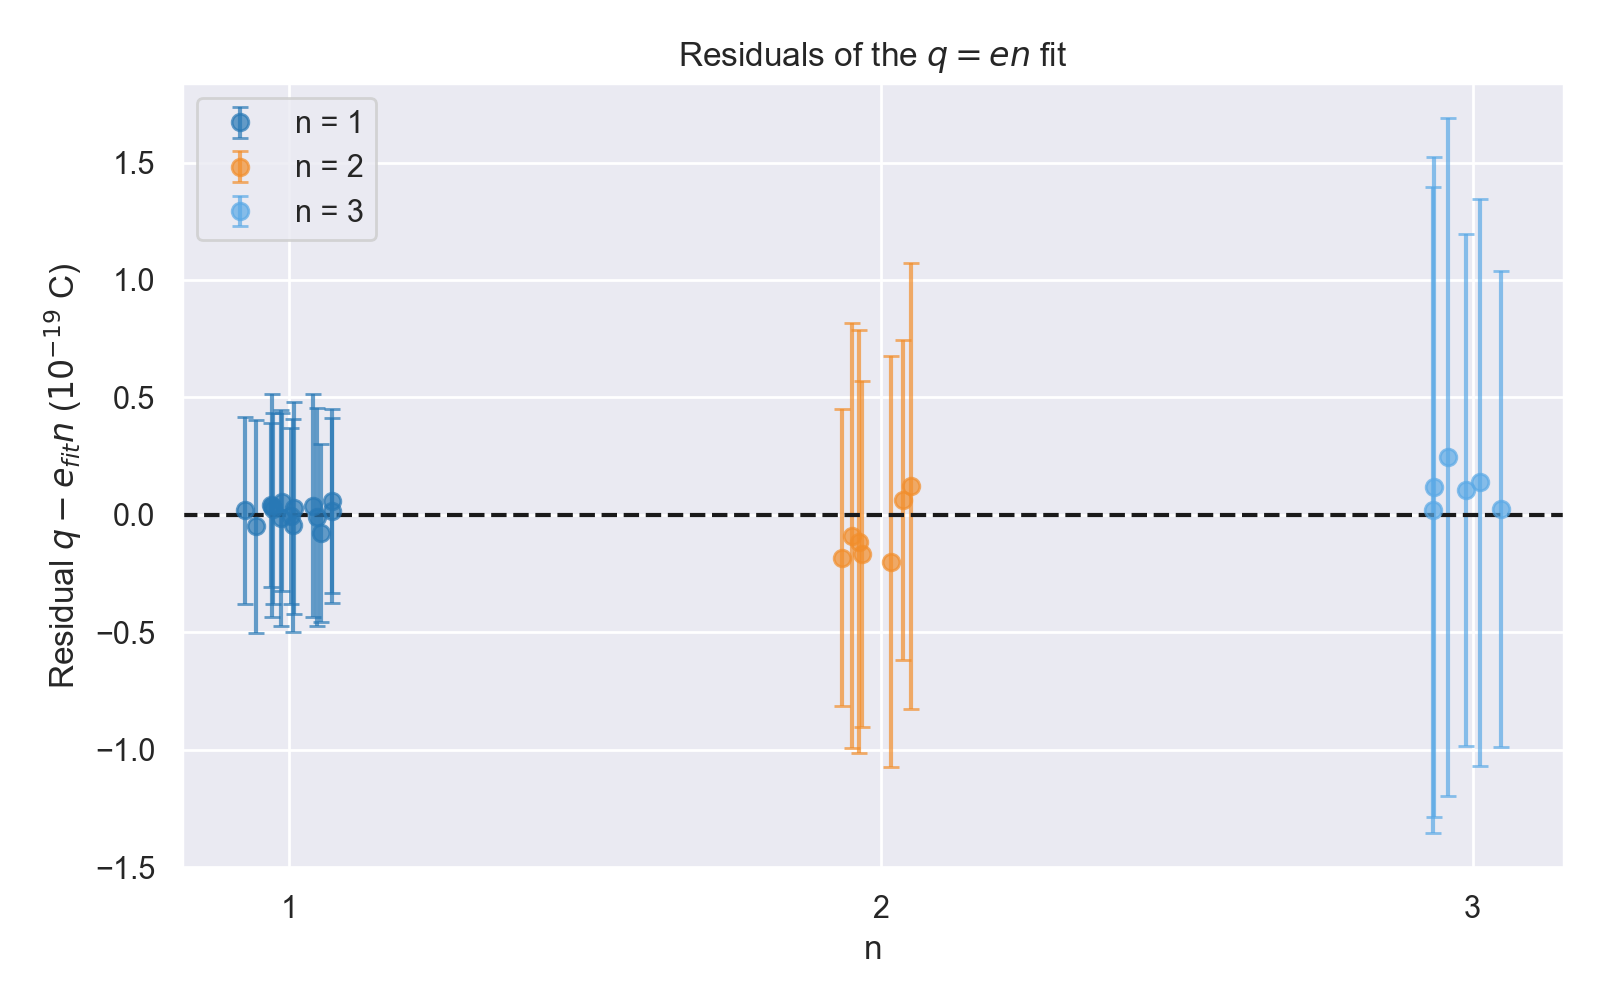
\includegraphics[width=0.8\textwidth]{images/Millikan_Residuals.png}
    \caption{Residuals $q-e_{\mathrm{fit}}n$ of the origin-constrained fit for
    each drop, with propagated uncertainties. The residuals scatter about zero
    with no systematic trend with $n$.}
    \label{fig:residuals}
\end{figure}

\begin{figure}[H]
    \centering
    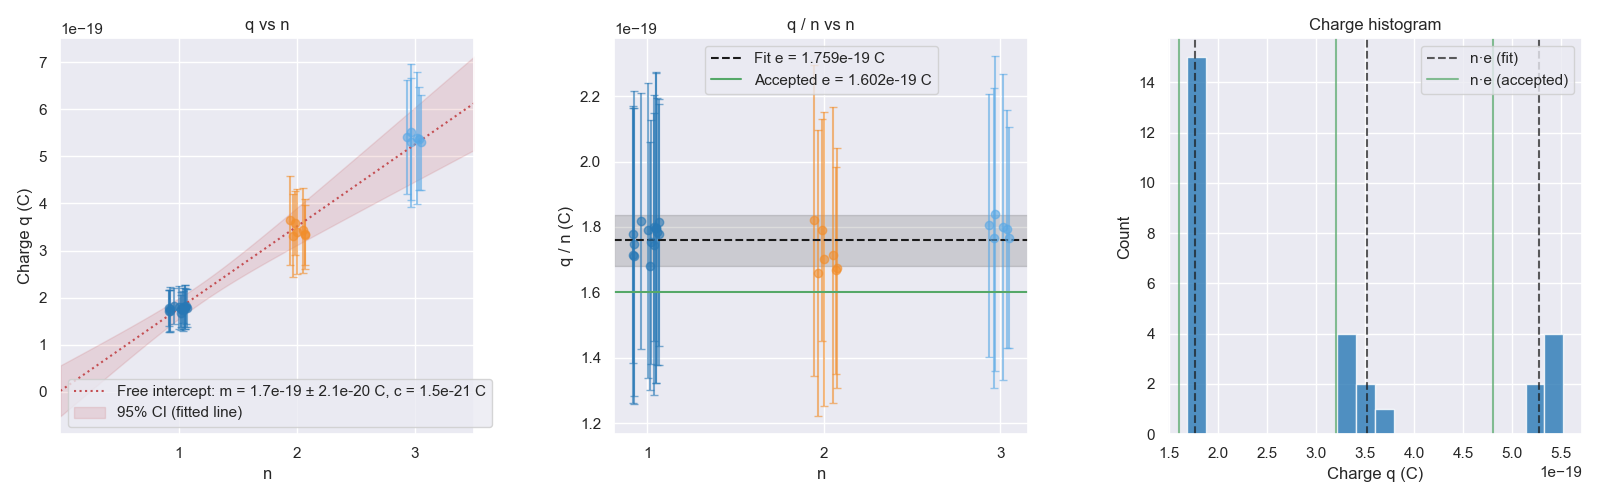
\includegraphics[width=0.8\textwidth]{images/Millikan_Combined_Analysis.png}
    \caption{Combined analysis of the Millikan experiment, showing the charge histogram, $q/n$ against $n$, and the residuals of the origin-constrained fit.}
    \label{fig:combined-analysis}
\end{figure}

The level estimates have a consistency statistic of $\chi^2=9.34$ for two
degrees of freedom. The weighted mean is $10.8\%$ above the accepted
elementary charge, $1.602176634\times10^{-19}\,\si{C}$; the origin-constrained
fit is $9.8\%$ high. The level statistic indicates more scatter between the
three level estimates than expected from their within-group standard errors.
The fit uncertainties instead use the propagated reading errors and common
pressure contribution, so they answer a different uncertainty question.

\subsection{Apparent-charge correction and revised $e_1$}

The apparent charge $q_{\mathrm{app}}$ is calculated before applying the slip correction with known A and the radius from Eq.~\ref{eq:radius}. Following Millikan's method, the true charge
$q$ and the apparent charge are related by

\begin{equation}
    q_{\mathrm{app}}^{2/3}
    = q^{2/3}\left(1+A\frac{\lambda}{r}\right)
    = n^{2/3}e_1^{2/3}\left(1+A\frac{\lambda}{r}\right),
    \qquad q=ne_1,
\end{equation}

so in terms of the apparent charge per unit, $e_{\mathrm{app}}=q_{\mathrm{app}}/n$,
the drops of every charge level lie on a single straight line,

\begin{equation}
    e_{\mathrm{app}}^{2/3}
    = e_1^{2/3}+e_1^{2/3}A\frac{\lambda}{r}
    = c+m\frac{\lambda}{r},
    \qquad c=e_1^{2/3},\quad m=cA .
\end{equation}
The intercept is $c=e_1^{2/3}$ and the slip constant is the
slope-to-intercept ratio, $A=m/c$.
The charges were assigned to levels $n=1,2,3$ by clustering the apparent
charges (15, 7 and 6 drops). All drops were fitted simultaneously with
a single line with two free parameters, $c=e_1^{2/3}$ and $m=cA$, and the
radius was recalculated self-consistently from the slip length $A\lambda$.
Figure~\ref{fig:qapp-lambda} shows the data, the fit and its residuals.
\begin{figure}[H]
    \centering
    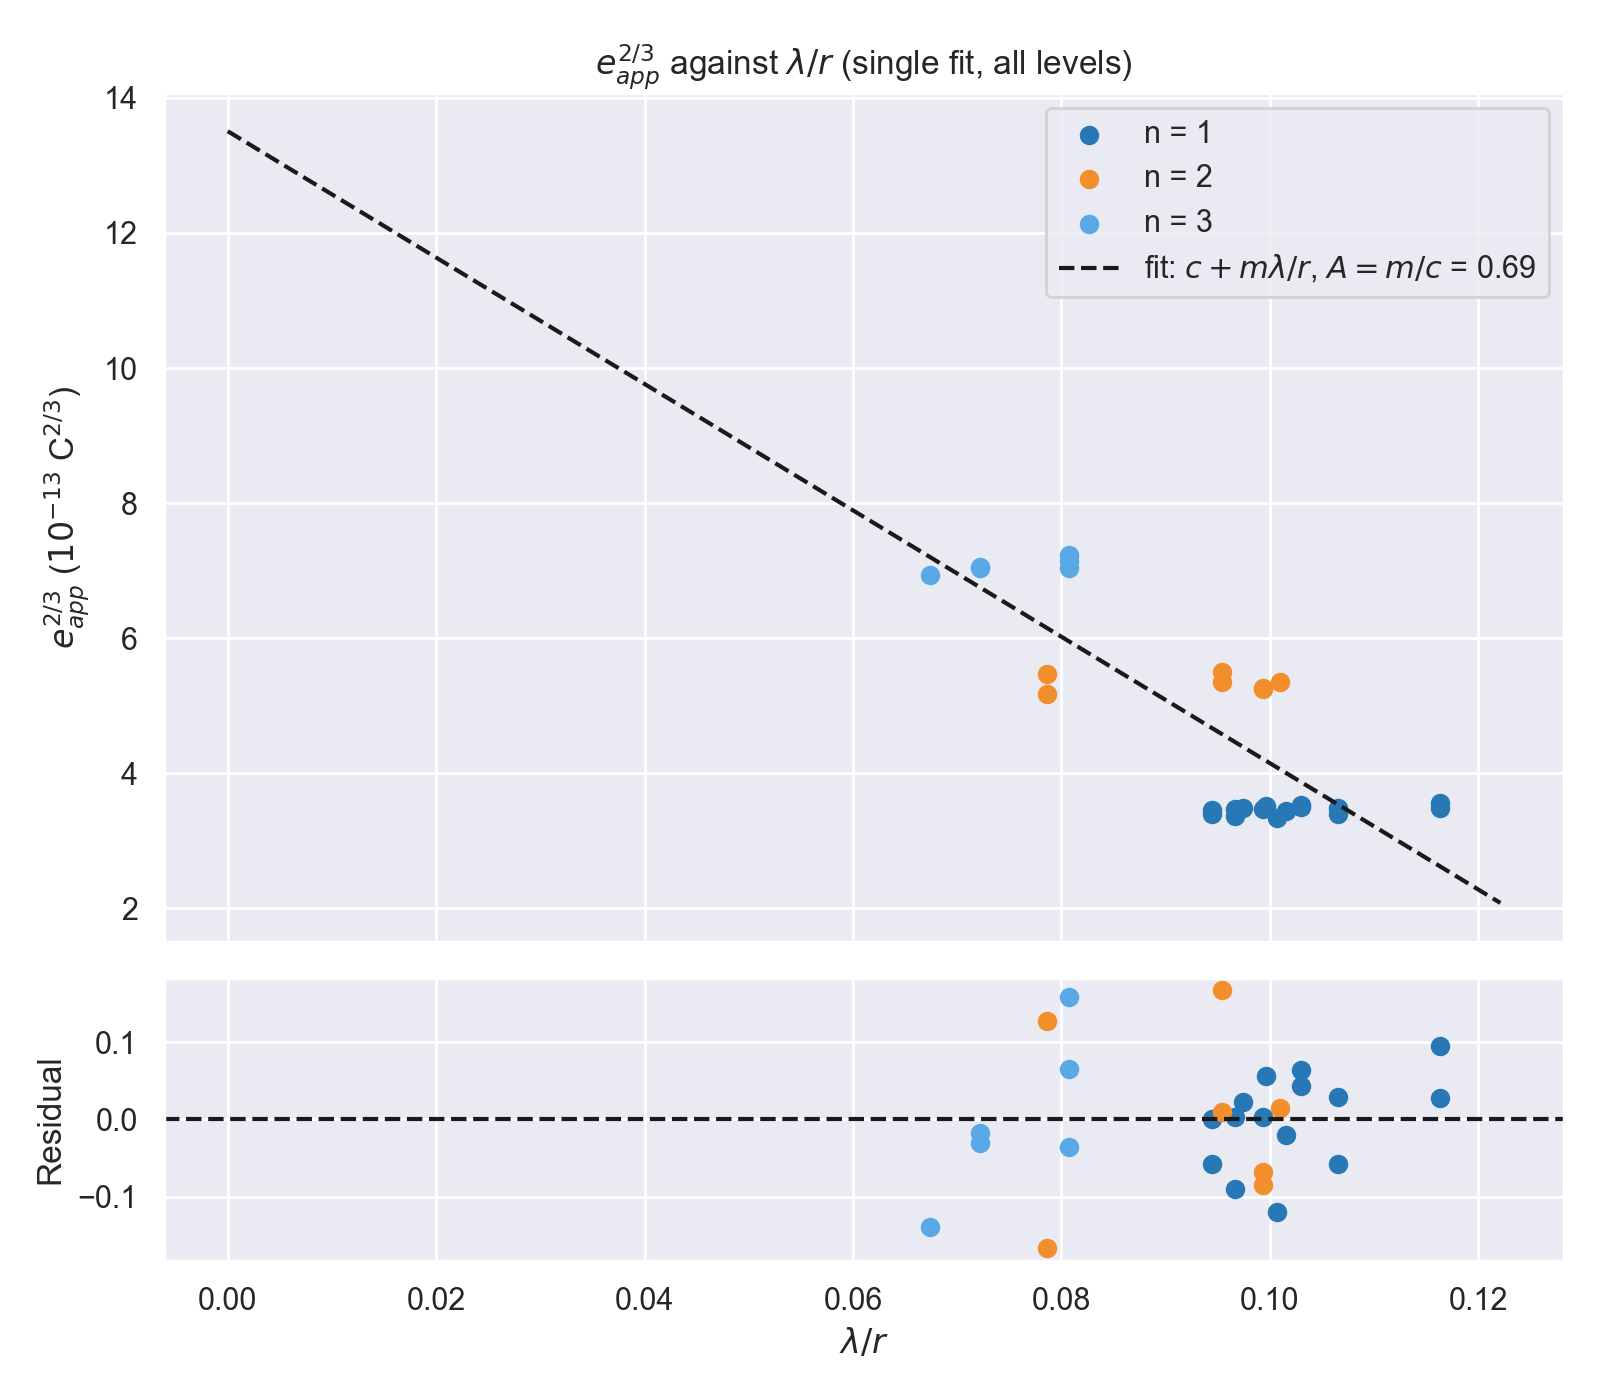
\includegraphics[width=0.8\textwidth]{images/Millikan_qapp_vs_lambda_over_r.png}
    \caption{$e_{\mathrm{app}}^{2/3}$ against $\lambda/r$ for all charge levels,
    with the single fit $c+m\lambda/r$ (dashed) and its residuals (lower
    panel).}
    \label{fig:qapp-lambda}
\end{figure}
The fitted $A$ is extremely weakly constrained because $\lambda/r$ spans only
$0.0674$--$0.1163$. The fit gives
\begin{equation}
    A_{\mathrm{fit}}=0.6927\pm0.55,\qquad
    A_{\mathrm{fit}}\lambda=4.6629\times10^{-8}\,\si{m}.
\end{equation}
The fitted intercept is
$c=(1.3506\times10^{-13}\pm2.63\times10^{-12})\,\si{C^{2/3}}$ and the slope is
$m=(0.936\pm458.753)\times10^{-13}\,\si{C^{2/3}}$. Using the reported
uncertainty $u_A=0.55$, the intercept implies
$e_1=(4.9633\times10^{-20}\pm1.45\times10^{-18})\,\si{C}$, but the fit
uncertainties are so large that this is not a useful estimate.

\paragraph{Analytic $A$.} Since $A\lambda=b/p$ and $\lambda\propto 1/p$, the
pressure cancels:
\begin{equation}
    A=\frac{b}{p\lambda}=\frac{\sqrt{2}\pi d^2 b}{k_{\mathrm{B}}T}
    =1.188\pm0.0004,
\end{equation}
using $b=8.0\times10^{-3}\,\si{Pa\,m}$ (Leybold), $d=\SI{0.370}{nm}$ and
$T=\SI{296.55}{K}$; the quoted uncertainty comes only from $u_T=\SI{0.1}{K}$
and excludes uncertainty in $b$ and $d$. The slip length is
$A\lambda=8.0\times10^{-8}\,\si{m}$. The fitted value is $0.583$ times the
analytic one, a difference of $0.9\sigma$ when the reported fit uncertainty
is used. The analytic $A$ is therefore adopted, and the free fit is treated
as a consistency check.

The apparent charges were corrected with the analytic $A$ using
\begin{equation}
    q_i=\frac{q_{\mathrm{app},i}}{(1+A\lambda/r_i)^{3/2}}.
\end{equation}
With $A$ fixed, the level estimates are:
\begin{center}
\begin{tabular}{lcc}
    \toprule
    Level & Measurements & $e_n$ ($10^{-19}\,\si{C}$) \\
    \midrule
    1 & 15 & $1.7148\pm0.0103$ \\
    2 & 7  & $1.6676\pm0.0232$ \\
    3 & 6  & $1.7420\pm0.0109$ \\
    \bottomrule
\end{tabular}
\end{center}
An unweighted least-squares fit of $q_n=ne_1$ to all 28 drops with $A$ fixed gives
\begin{equation}
    e_1=(1.72\pm0.01)\times10^{-19}\,\si{C}.
\end{equation}
The uncertainty is the statistical uncertainty from the scatter about the fit; it does not include
uncertainty in $A$, $b$, the molecular diameter, or shared apparatus
constants. Freeing $A$ gives
$e_1=(4.9633\times10^{-20}\pm1.45\times10^{-18})\,\si{C}$
($-69.0\%$ relative to the accepted value), but the uncertainty is much larger
than the estimate itself; this result is not a useful measurement.

\newpage

%================================================
\section{Error Analysis}
%================================================

The falling and rising speeds were recalculated from the measured travel
distance $s$ and time $t$ using $v=s/t$. A graticule division is
\SI{0.5}{mm}; the recorded integer division counts were assigned a reading
uncertainty of half a division, $u_s=\SI{0.25}{mm}$. Time and voltage
uncertainties were taken as half the last recorded digit. Assuming independent
uncertainties in distance and time, the speed uncertainty is
\begin{equation}
    u_v^2 =
    \left(\frac{\partial v}{\partial s}u_s\right)^2
    +\left(\frac{\partial v}{\partial t}u_t\right)^2
    =
    \left(\frac{u_s}{t}\right)^2
    +\left(\frac{s\,u_t}{t^2}\right)^2,
\end{equation}
or, equivalently,
\begin{equation}
    \left(\frac{u_v}{v}\right)^2 =
    \left(\frac{u_s}{s}\right)^2
    +\left(\frac{u_t}{t}\right)^2.
\end{equation}
This calculation was applied separately to the falling speed $v_g$ and the
rising speed $v_E$. A missing rising-time measurement represents a stationary
drop; in that case $v_E$ and its uncertainty were set to zero.

For each drop, the charge was calculated using
\begin{equation}
    q = \frac{q_0}{C_{\mathrm{c}}^{3/2}},
    \qquad
    C_{\mathrm{c}} = 1+\frac{A}{r},
    \qquad
    A=\frac{b}{p},
\end{equation}
where $q_0$ and the corrected radius $r$ are given in the Theory section.
The charge depends on the measured and apparatus quantities
\begin{equation}
    \boldsymbol{x} =
    (d,V,\eta,\rho,v_g,v_E,p,b).
\end{equation}
For independent input uncertainties, the propagated charge uncertainty is
\begin{equation}
    u_q^2 =
    \sum_j
    \left(
        \frac{\partial q}{\partial x_j}u_{x_j}
    \right)^2.
    \label{eq:charge-uncertainty}
\end{equation}
The derivatives in Equation~\ref{eq:charge-uncertainty} include the
dependence of both $r$ and $C_{\mathrm{c}}$ on the input quantities. They
were evaluated numerically using central finite differences. For this
calculation, $d=\SI{6}{mm}$, $\eta=\SI{1.83e-5}{Pa.s}$,
$\rho=\SI{900}{kg.m^{-3}}$, and $b=\SI{8.0e-3}{Pa.m}$ were treated as exact;
the nonzero apparatus uncertainty was $u_p=\SI{4}{hPa}$. Thus these results
are a propagated reading-and-pressure budget, not a complete budget including
uncertainties in the exact-treated constants. Since pressure is shared by all
measurements, the corresponding covariance terms were included in the fits:
\begin{equation}
    u_q^2 =
    \sum_j\sum_k
    \frac{\partial q}{\partial x_j}
    \frac{\partial q}{\partial x_k}
    \operatorname{Cov}(x_j,x_k).
\end{equation}

Before applying the slip correction, the uncorrected charge has the relative
uncertainty
\begin{align}
    \left(\frac{\sigma_{q_0}}{q_0}\right)^2 ={}&
    \left(\frac{\sigma_d}{d}\right)^2
    +\left(\frac{\sigma_V}{V}\right)^2
    +\left(\frac{3\sigma_\eta}{2\eta}\right)^2
    +\left(\frac{\sigma_\rho}{2\rho}\right)^2
    +\left(\frac{\sigma_g}{2g}\right)^2 \nonumber\\
    &+\left[
        \left(
            \frac{1}{v_g+v_E}+\frac{1}{2v_g}
        \right)\sigma_{v_g}
    \right]^2
    +\left(\frac{\sigma_{v_E}}{v_g+v_E}\right)^2 .
    \label{eq:uncorrected-charge-uncertainty}
\end{align}
This expression is for $q_0$ only; the final uncertainty in $q$ must also
account for the Cunningham correction through the full propagation above.

For each charge level, the mean charge and its standard error were calculated
from the $N$ recomputed charges in that group:
\begin{equation}
    \bar{q} = \frac{1}{N}\sum_{i=1}^{N}q_i,
    \qquad
    \sigma_{\bar{q},\mathrm{stat}} =
    \frac{s_q}{\sqrt{N}},
    \qquad
    s_q =
    \sqrt{\frac{1}{N-1}\sum_{i=1}^{N}(q_i-\bar{q})^2}.
\end{equation}
For a group assigned level $n$, the elementary-charge estimate and its
statistical uncertainty are
\begin{equation}
    e_n = \frac{\bar{q}}{n},
    \qquad
    \sigma_{e_n,\mathrm{stat}} = \frac{\sigma_{\bar{q},\mathrm{stat}}}{n}.
\end{equation}
These standard errors describe the scatter of the measurements within each
group. They do not include shared systematic uncertainties, such as
uncertainty in the plate separation or voltage. Any such contributions
should be reported separately and should not be reduced by $1/\sqrt{N}$.

If the level estimates are independent and only their statistical
uncertainties are combined, the inverse-variance weighted estimate is
\begin{equation}
    e_{\mathrm{weighted}} =
    \frac{\displaystyle\sum_n e_n/\sigma_{e_n,\mathrm{stat}}^2}
         {\displaystyle\sum_n 1/\sigma_{e_n,\mathrm{stat}}^2},
    \qquad
    \sigma_{e,\mathrm{weighted}} =
    \left(\sum_n \frac{1}{\sigma_{e_n,\mathrm{stat}}^2}\right)^{-1/2}.
\end{equation}

The percentage difference from the accepted elementary charge is
\begin{equation}
    \text{percentage difference} =
    \frac{|e_{\mathrm{measured}}-e_{\mathrm{accepted}}|}
         {e_{\mathrm{accepted}}}\times100\%.
\end{equation}

\subsection{Uncertainty on $e_1$ from the expected $A$.}
Using the expected value of $A$, the uncertainty in $e_1$ can be propagated from Eq.~\ref{eq:uncorrected-charge-uncertainty},
\[
    \sigma_{e_1} = 1.7 \pm 0.1 \si{C}.
\]


\subsection{Uncertainty on $e_1$ from the fitted $A$.}
The Cunningham fit is $e_{\mathrm{app}}^{2/3}=c+m\lambda/r$ with
$c=e_1^{2/3}$ and $A=m/c$. Its parameters and covariance come from the
least-squares Jacobian, scaled by the residual variance. This gives
$c=(1.3506\times10^{-13}\pm2.63\times10^{-12})\,\si{C^{2/3}}$,
$m=(0.936\pm458.753)\times10^{-13}\,\si{C^{2/3}}$, and
$A=0.6927\pm0.55$. Since $e_1=c^{3/2}$, propagating $u_c$ gives
\begin{equation}
    \sigma_{e_1}=\frac{3}{2}\,c^{1/2}\,u_c=\frac{3}{2}\,e_1\frac{u_c}{c},
\end{equation}
so
\begin{equation}
    e_1=(4.9633\times10^{-20}\pm1.45\times10^{-18})\,\si{C},
\end{equation}
which is $69.0\%$ below the accepted value, but is not a useful estimate
because its uncertainty is much larger than its central value. With the
analytic $A$ the unweighted fit gives
$e_1=(1.72\pm0.01)\times10^{-19}\,\si{C}$, but that error has no
contribution from $A$, $b$ or $d$, so it is optimistic. As above, the quoted
uncertainties exclude the exact-treated constants.
\newpage

%================================================
\section{Discussion}

\subsection{Quantisation of charge}
The central result is that the apparent charges do not form a continuum. The
$28$ drops fall into three well separated groups, with weighted means
$q_1\approx1.77$, $q_2\approx3.44$ and $q_3\approx5.39$ in units of
$10^{-19}\,\si{C}$. These stand in the ratio $1:1.94:3.05$, close to
$1:2:3$, so each drop carries a small whole number of a single fundamental
unit. A fit of $q=en+c$ is consistent with a zero intercept, as expected if
no charge is carried by a drop with $n=0$. No drop was found between the
groups, even though the oil droplets were charged by friction in an
uncontrolled way, so a continuous charge distribution would populate the
gaps. This is the key conclusion of Millikan's experiment: charge is
quantised, and the value of the unit $e$ can be read from the spacing
of the levels.

The experiment supports this, but does not prove it beyond doubt. The level
estimates have $\chi^2=9.34$ for two degrees of freedom, so the spread
between groups is larger than the within-group standard errors imply. The
likely cause is uncertainty not in the error budget (drop radius, viscosity,
a small error in the assigned $n$ for individual drops), rather than a failure
of quantisation. Only three levels were reached, and the $n=3$ group has
few drops with large individual uncertainties.

\subsection{Brownian motion and the slip correction}
The drops have radii of order $\SI{e-6}{m}$, comparable with the mean free
path of air, $\lambda\approx\SI{7e-8}{m}$, so $\lambda/r\approx0.07$--$0.11$.
The air therefore cannot be treated as a continuous fluid: the drop is
bombarded by individual molecules, which is the same molecular bombardment
that produces Brownian motion. Two consequences appear in the data.
First, the Cunningham slip correction is expected from the molecular nature
of air, and applying the analytic correction shifts the three level estimates.
However, the fitted slope is too uncertain here to measure this effect
independently. Second, the random molecular impacts
make the measured fall and rise times fluctuate from one passage to the next,
which contributes to the scatter of the speeds and hence of the charges. The
experiment is therefore an exploration of Brownian motion as well as of
charge quantisation: the slip correction tests the kinetic picture of a gas,
and the transit-time scatter is the Brownian noise on the terminal velocity.

\subsection{Success of the experiment and Avogadro's number}
The experiment was successful in its main aims. It shows clearly grouped
charges and gives $e_1=(1.7\pm0.1)\times10^{-19}\,\si{C}$ if the
analytic $A$ is used, which is $7.1\%$ above the accepted value of
$1.602\times10^{-19}\,\si{C}$. The free fit gives
$A=0.6927\pm0.55$, consistent with the analytic value within $0.9\sigma$.
Its central value corresponds to $n=1.4236\times10^{25}\,\si{m^{-3}}$ and
Avogadro's number
(Appendix, Section on Avogadro's Number),
\[
N_{\mathrm{A}}=(3.51\pm2.79)\times10^{23}\,\si{mol^{-1}},
\]
whose central value is $41.7\%$ below $6.022\times10^{23}\,\si{mol^{-1}}$,
but consistent within $0.9\sigma$. Thus, the experiment estimates the charge
of the electron from the grouped drop charges and gives a rough independent
estimate of Avogadro's number. This is the same link made by Einstein's and
Perrin's analysis of Brownian motion~\cite{Einstein1905}~\cite{Perrin1914},
where $N_{\mathrm{A}}=R/k_{\mathrm{B}}$ is fixed by the thermal motion of
small particles. Using the analytic $A$ returns $N_{\mathrm{A}}$ exactly, but
that is circular, so only the fitted-$A$ value is an independent result.

\subsection{Limitations}
The measured values of $e_1$ are high. The weighted level estimate is
$10.8\%$ above the accepted elementary charge, and the origin-constrained fit
is $9.8\%$ high. The propagated uncertainties treat plate spacing,
viscosity, oil density, the slip constant and the molecular diameter as exact,
so they do not capture calibration uncertainty in these quantities. A shared
scale error would affect all drops alike; since $q\propto\eta^{3/2}$, a
few-percent error in $\eta$ (which varies with temperature) would shift $e_1$
by more than that. The data does not identify which systematic effect, if any,
explains the difference. The calculation also assumes spherical drops,
terminal motion, a uniform field between the plates and the stated
Cunningham correction; departures from these are not in the reading
uncertainties. The low reduced chi-squared of the individual-point fits
should be read in light of the assumed reading resolutions and omitted
calibration terms, not as independent confirmation of the uncertainty
model. The $N_{\mathrm{A}}$ uncertainty comes only from $A_{\mathrm{fit}}$ and
omits $d$ and $b$, on which it depends strongly ($\propto 1/d^2b$).

\newpage

%================================================
\section{Conclusion}

The analytic Cunningham coefficient is $A=\sqrt{2}\pi d^2 b/(k_{\mathrm{B}}T)=1.188$.
Millikan's method of fitting $q_{\mathrm{app}}^{2/3}$ against $\lambda/r$ gives
$A=0.6927\pm0.55$, consistent with the analytic value within $0.9\sigma$.
Correcting the apparent charges with the analytic $A$ gives
$e_1=(1.7\pm0.1)\times10^{-19}\,\si{C}$, which is $7.1\%$ above the
accepted value. The free fit is too uncertain to give a useful alternative
estimate. This result supports charge grouping, while a full uncertainty
budget must also include uncertainty in $b$, the molecular diameter and shared
apparatus constants.


%================================================

\newpage

%================================================
\section{References}
%================================================
\printbibliography
%================================================

\newpage

%================================================
\appendix
\section{Appendix}
\subsection{Cunningham correction factor}
\label{app:cunningham}

The Cunningham correction factor accounts for the slip of air molecules around
small particles, which affects the drag force experienced by the oil drops.
A general empirical form is

\begin{equation}
    C_{\mathrm{c}} = 1 + \frac{\lambda}{r}
    \left(\alpha + \beta\exp\left(-\frac{\gamma r}{\lambda}\right)\right),
\end{equation}

where $\lambda$ is the mean free path of air molecules, $r$ is the drop
radius, and $\alpha$, $\beta$, and $\gamma$ are empirical constants. For the
calculations in this report, the Leybold apparatus approximation is used:

\begin{equation}
    C_{\mathrm{c}}(r,p) = 1 + \frac{b}{rp}
    = 1 + \frac{A}{r},
    \qquad A=\frac{b}{p},
\end{equation}

with $b=80\,\mu\mathrm{m\,hPa}$ for the apparatus and air pressure $p$.
This is the correction used in the drag and charge calculations in the main
text. Here $b/p=A\lambda$, so $A=b/(p\lambda)$ is the dimensionless coefficient
used in the main text, and $\lambda/r$ is the Knudsen-type ratio. The linear
form is the first-order slip expansion; for $\lambda/r=0.0674$--$0.1163$ in this
experiment the exponential term in the general form is negligible. The
coefficient $b$ depends on gas--surface accommodation and is an empirical,
apparatus-quoted constant (Leybold $b=8.0\times10^{-3}\,\si{Pa\,m}$ versus the
slightly different value quoted in the Oxford notes), so it cannot be derived
exactly from the Knudsen number alone. The general form has the empirical
coefficients $\alpha,\beta,\gamma$ in place of the single $A$.

\subsection{Derivation of the fit model and analytic $A$}

Terminal-velocity motion with slip gives a Stokes drag reduced by
$1+A\lambda/r$, so the apparent radius $r_0$, computed without slip, obeys
\begin{equation}
    r_0^2=r^2+A\lambda r
    \;\Rightarrow\;
    r=\sqrt{r_0^2+\tfrac{(A\lambda)^2}{4}}-\tfrac{A\lambda}{2},
\end{equation}
and the charge scales as $q\propto r^{3/2}$ at fixed velocity ratio, giving
$q_{\mathrm{app}}^{2/3}=q^{2/3}(1+A\lambda/r)$ as used in the Analysis. The fit
minimises the residuals of this relation over all 28 drops with one $A$
and one $e_1^{2/3}$. Using $\lambda=k_{\mathrm{B}}T/(\sqrt{2}\pi d^2p)$,
\begin{equation}
    A=\frac{b}{p\lambda}=\frac{\sqrt{2}\pi d^2 b}{k_{\mathrm{B}}T},
\end{equation}
so the pressure cancels. The uncertainty of the free fit was estimated from
the least-squares covariance scaled by the residual variance.

\subsection{Mean Free Path of Air Molecules}

The mean free path of air molecules, denoted by $\lambda$, is the average distance a molecule travels between collisions. It is given by the expression:

\begin{equation}
    \lambda = \frac{k_{\mathrm{B}} T}{\sqrt{2} \pi d^2 p},
    \label{eq:mean_free_path}
\end{equation}

where $k_{\mathrm{B}}$ is the Boltzmann constant, $T$ is the absolute temperature, $d$ is the effective diameter of an air molecule, and $p$ is the air pressure. This parameter is crucial for calculating the Cunningham correction factor for small oil drops.

Using $T=\SI{296.55}{K}$, $p=\SI{1000}{hPa}$, and an effective air-molecule
diameter $d=\SI{0.370}{nm}$ gives the mean free path

\[
    \lambda = 6.7315\times10^{-8}\,\si{m}.
\]

\subsection{Calculating Avogadro's Number}

For molecules of diameter $d$, the collision cross-section is
$\pi d^2$. In a gas with number density $n$, the mean free path,
neglecting the relative motion of molecules, is
\[
\lambda_0 = \frac{1}{n\pi d^2}.
\]
Accounting for the relative motion introduces a factor of $\sqrt{2}$,
giving
\[
\lambda = \frac{1}{\sqrt{2}\,n\pi d^2},
\]
consistent with Eq.~\ref{eq:mean_free_path}, where
$n=p/(k_{\mathrm{B}}T)$.

Avogadro's number is related to the number density by
\[
N_{\mathrm{A}} = nV_{\text{molar}},
\]
where $V_{\text{molar}}=RT/p$ is the molar volume of an ideal gas.
Using the slip-correction constant $A=b/(p\lambda)$, we obtain
\[
\lambda = \frac{b}{pA},
\qquad
n = \frac{pA}{\sqrt{2}\,\pi d^2b}.
\]
Substituting this expression into the equation for $N_{\mathrm{A}}$
eliminates the pressure, yielding
\[
\boxed{
N_{\mathrm{A}} = \frac{ART}{\sqrt{2}\,\pi d^2b}
}.
\]

Using $R=\SI{8.3145}{J.mol^{-1}.K^{-1}}$,
$T=\SI{296.55}{K}$, $d=\SI{0.370}{nm}$, and
$b=8.0\times10^{-3}\,\si{Pa.m}$, together with the fitted value
$A=0.6927\pm0.55$, gives
\[
\lambda = 1.1549\times10^{-7}\,\si{m},
\qquad
n = 1.4236\times10^{25}\,\si{m^{-3}}.
\]
The resulting estimate of Avogadro's number is
\[
\boxed{
N_{\mathrm{A}} = (3.51\pm2.79)\times10^{23}\,\si{mol^{-1}}
}.
\]
The central value is $41.7\%$ below the accepted value of
$6.022\times10^{23}\,\si{mol^{-1}}$~\cite{Perrin1914}, but remains
consistent with it within $0.9\sigma$.

The quoted uncertainty accounts only for the uncertainty in
$A_{\text{fit}}$; it excludes uncertainties in $d$ and $b$, on which
the estimate depends strongly, with
$N_{\mathrm{A}}\propto 1/(d^2b)$ for fixed $A$.

For comparison, substituting the analytic value $A=1.188$ reproduces
the accepted value of $N_{\mathrm{A}}$. However, this agreement is
circular rather than an independent measurement: since
$A\propto d^2b/(k_{\mathrm{B}}T)$, substitution reduces the expression
to $N_{\mathrm{A}}=R/k_{\mathrm{B}}$. The result therefore serves only
as a consistency check, not an independent determination of
Avogadro's number~\cite{millikan1917electron}.

\end{document}
%================================================
